\documentclass{beamer}

\mode<presentation> {
\usetheme{Madrid} %Default - Use this
\usecolortheme{whale}
}

%%%%%%%%%%% To Set the reference to black color (Default is blue color for this theme )
\setbeamertemplate{bibliography item}[text] % For IEEE Format citations
\setbeamercolor{bibliography item}{fg=black} 
\setbeamercolor{bibliography entry author}{fg=black}
\setbeamercolor{bibliography entry title}{fg=black} 
\setbeamercolor{bibliography entry location}{fg=black} 
\setbeamercolor{bibliography entry note}{fg=black}


\usepackage{graphicx}
  \DeclareGraphicsExtensions{.pdf,.jpeg,.png,.eps,.jpg}
\usepackage{subcaption} 
\usepackage{booktabs} % Allows the use of \toprule, \midrule and \bottomrule in tables
\usepackage{multirow} % For multirow table
\usepackage{amssymb,amsmath,bm}
\usepackage{amsmath}
\usepackage[para]{threeparttable}
\usepackage{epstopdf}
\usepackage{tikz}
\usetikzlibrary{shapes,arrows}
\usepackage{media9}
\usepackage{hyperref}
\usepackage{longtable}
\usepackage{multirow}
\usepackage{pdfpages}
%\usepackage{fancyvrb} % For verbatim
%\usepackage{fixltx2e}

%\usepackage[font=Helv,timeinterval=10]{tdclock}
%\setbeamertemplate{headline}{\initclock\tiny{\cronominutes\pdfcolon\cronoseconds}}


%----------------------------------------------------------------------------------------
%	TITLE PAGE
%----------------------------------------------------------------------------------------

\title[Progress Seminar]{Indexing and Retrieval of Video Lectures} 

\author[Narayan Kunal]{
{\footnotesize{Progress Seminar} \\ 
{\textit{by}} \\ 
\textbf{{Narayan Kunal} \\
{Roll No. 18CS60R56 }}\\ \vspace*{3mm}
%\begin{figure}

\includegraphics[width=0.15\linewidth]{figures/iit_kgp_80} \\ \vspace*{3mm} % For Blue Color
%\includegraphics[width=0.1\linewidth]{figures/iitlogo} \\ \vspace*{3mm} % For Black Color
%\end{figure}
{\textit{under the supervision of}}\\ \vspace*{2mm}
\textbf{{Prof. K Sreenivasa Rao }} \\ \vspace*{1mm}
{\bf{Department of Computer Science and Engineering\\ Indian Institute of Technology Kharagpur}}
}
}

\date{\today} % Date, can be changed to a custom date


\begin{document}
\begin{frame}
\titlepage % Print the title page as the first slide
\end{frame}

\begin{frame}
\frametitle{Overview} 
\tableofcontents 
\end{frame}

\tikzstyle{block} = [draw, fill=blue!20, rectangle, 
    minimum height=3em, text width=5em, text centered, rounded corners]
\tikzstyle{sum} = [draw, fill=blue!20, circle, node distance=1cm]
	\tikzstyle{pinstyle} = [pin edge={to-,thin,black}]
\tikzstyle{block1} = [draw, fill=blue!20, rectangle, 
    minimum height=3em, text width=10em, text centered, rounded corners]
\tikzstyle{decision} = [draw, fill=blue!20, diamond, 
    minimum width=3cm, minimum height=1cm, text centered, aspect=1.5]
\tikzstyle{arrow} = [thick,->,>=stealth]

%----------------------------------------------------------------------------------------
%	PRESENTATION SLIDES
%----------------------------------------------------------------------------------------


%%%%%%%%%%%%%%%%%%%%%%%%%%%%%%%%%%%%%%%%%%%%%%%%%%%%%%%%%%%%%%%%%%%%%%%%%%%%%%%%%%%%%%%%%
\section{Introduction} \label{Introduction}

\begin{frame}
\frametitle{Introduction}
\begin{itemize}
	
	\item Digital video has become a popular storage and exchange medium due to the rapid development in recording technology, improved video compression techniques and high-speed networks in the last few years. 
	
	\item As a result, there has been a huge increase in the amount of multimedia data on the Web. Therefore, for a user it is nearly impossible to find desired videos without a search function  within a video archive.
	
	\item The requested information may be covered in only a few minutes, the user might thus want to find the piece of information he requires without viewing the complete video.

\end{itemize}
\end{frame}

%%%%%%%%%%%%%%%%%%%%%%%%%%%%%%%%%%%%%%%%%%%%%%%%%%%%%%%%%%%%%%%%%%%%%%%%%%%%%%%%%%%%%%%%%
\section{Objective} \label{Objective}

\begin{frame}
\frametitle{Objective}
\begin{itemize}
	
	\item Most of the video retrieval and video search systems such as YouTube, Bing and Vimeo rely on available textual metadata such as title, genre, person, and brief description, etc. 
	\item Generally, this kind of metadata has to be created by a human to ensure a high quality, but the creation step is rather time and cost consuming.
	\item Our target is to generate metadata automatically using video analysis tool.
	
\end{itemize}
\end{frame}

%%%%%%%%%%%%%%%%%%%%%%%%%%%%%%%%%%%%%%%%%%%%%%%%%%%%%%%%%%%%%%%%%%%%%%%%%%%%%%%%%%%%%%%%%

\section{Experimental Setup} \label{Experimental Setup}
\begin{frame}
\frametitle{Experimental Setup}
	\begin{itemize}
		\item Course Details
		\begin{itemize}
			\item Name : Cloud Computing
			\item Instructor : Prof Soumya Kanti Ghosh
			\item Institute : IIT Kharagpur
			\item Link : \url{https://nptel.ac.in/courses/106105167/}
			\item Numbers of lectures : 40
		\end{itemize}
		\item Tools used
		\begin{itemize} 
			\item OpenCV for video processing
			\item Pytesseract for OCR
		\end{itemize}
	\end{itemize}
\end{frame}
%%%%%%%%%%%%%%%%%%%%%%%%%%%%%%%%%%%%%%%%%%%%%%%%%%%%%%%%%%%%%%%%%%%%%%%%%%%%%%%%%%%%%%%%%
\section{Terminology} \label{Terminology}
\begin{frame}
\frametitle{Terminology}
	\begin{itemize}
		\item Mean Square Error(MSE) : MSE is the cumulative squared error between the two frame F1 and F2.
		\begin{center}
			$MSE(F1,F2) = \frac{1}{MN}\sum_{n=1}^{M}\sum_{m=1}^{N}[F2(n,m)-F1(n,m)]^2$
		\end{center}
		\item Manhattan Distance : The manhattan distance is the simple sum of the
		horizontal and vertical components.
		\begin{center}
			$MH(a,b) = |x_1-y_1|+|x_2-y_2|+...+|x_n-y_n|$
			\\where $a = (x_1,x_2,x_3,...,x_n) , b=(y_1,y_2,y_3,...,y_n)$
		\end{center}
		\item Euclidean Distance : It is the straight-line distance between two pixels.  the euclidean distance
		between two points $a = (a_x, a_y)$ and $b = (b_x, b_y)$ is defined as :
		\begin{center}
			$d(a,b) = \sqrt{(b_x-a_x)^2+(b_y-a_y)^2}$
		\end{center}
	\end{itemize}
\end{frame}
%%%%%%%%%%%%%%%%%%%%%%%%%%%%%%%%%%%%%%%%%%%%%%%%%%%%%%%%%%%%%%%%%%%%%%%%%%%%%%%%%%%%%%%%%
\begin{frame}
\frametitle{Terminology(contd..)}
\begin{figure}
	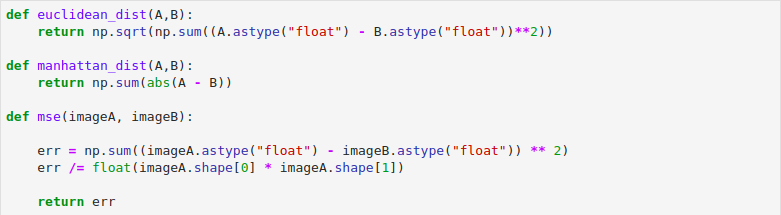
\includegraphics[width=0.9\linewidth, height=0.4\textheight]{Presentation_Image/code}
	\caption{Python Code}
	\label{fig:code}
\end{figure}
	
\end{frame}
%%%%%%%%%%%%%%%%%%%%%%%%%%%%%%%%%%%%%%%%%%%%%%%%%%%%%%%%%%%%%%%%%%%%%%%%%%%%%%%%%%%%%%%%%%
\section{Ground Truth}
\begin{frame}
\frametitle{Ground Truth}
	\begin{itemize}
		\item This ground truth is from 15 minute clip of Lecture 6 of cloud computing. All analysis has been done based on this.
	\end{itemize}
\begin{table}[]
	\begin{tabular}{|c|c|c|c|c|c|c|c|}
		\hline
		Time & 00:00 & 00:01 & 00:08 & 01:25 & 01:51 & 02:54 & 03:51 \\ \hline
		Slide No   & 1     & 2     & 3     & 4     & 5     & 6     & 7     \\ \hline
	\end{tabular}
\end{table}

\begin{table}[]
	\begin{tabular}{|c|c|c|c|c|c|c|c|}
		\hline
		Time & 04:11 & 04:13 & 04:57 & 05:19 & 05:27 & 06:21 & 06:23 \\ \hline
		Slide No   & 8     & 9     & 10    & 11    & 12    & 13    & 14    \\ \hline
	\end{tabular}
\end{table}

\begin{table}[]
	\begin{tabular}{|c|c|c|c|c|c|c|c|}
		\hline
		Time & 07:11 & 07:38 & 07:43 & 08:49 & 08:50 & 08:53 & 09:02 \\ \hline
		Slide No   & 15    & 16    & 17    & 18    & 19    & 20    & 21    \\ \hline
	\end{tabular}
\end{table}

\begin{table}[]
	\begin{tabular}{|c|c|c|c|c|c|c|c|c|}
		\hline
		Time & 09:24 & 09:56 & 10:02 & 10:56 & 11:42 & 11:47 & 13:56 & 14:11 \\ \hline
		Slide No   & 22    & 23    & 24    & 25    & 26    & 27    & 28    & 29    \\ \hline
	\end{tabular}
	\caption{Slide Number vs Timestamp}
\end{table}

\end{frame}
%%%%%%%%%%%%%%%%%%%%%%%%%%%%%%%%%%%%%%%%%%%%%%%%%%%%%%%%%%%%%%%%%%%%%%%%%%%%%%%%%%%%%%%%%

%%%%%%%%%%%%%%%%%%%%%%%%%%%%%%%%%%%%%%%%%%%%%%%%%%%%%%%%%%%%%%%%%%%%%%%%%%%%%%%%%%%%%%%%%
\section{Slide Extraction}
\begin{frame}
\frametitle{Slide Example}
\begin{figure}[h!]
	\centering
	\begin{subfigure}[b]{0.45\linewidth}
		
\includegraphics[width=\linewidth]{Presentation_Image/topic.jpg}
	\end{subfigure}
	\caption{Topic}
	\begin{subfigure}[b]{0.45\linewidth}
		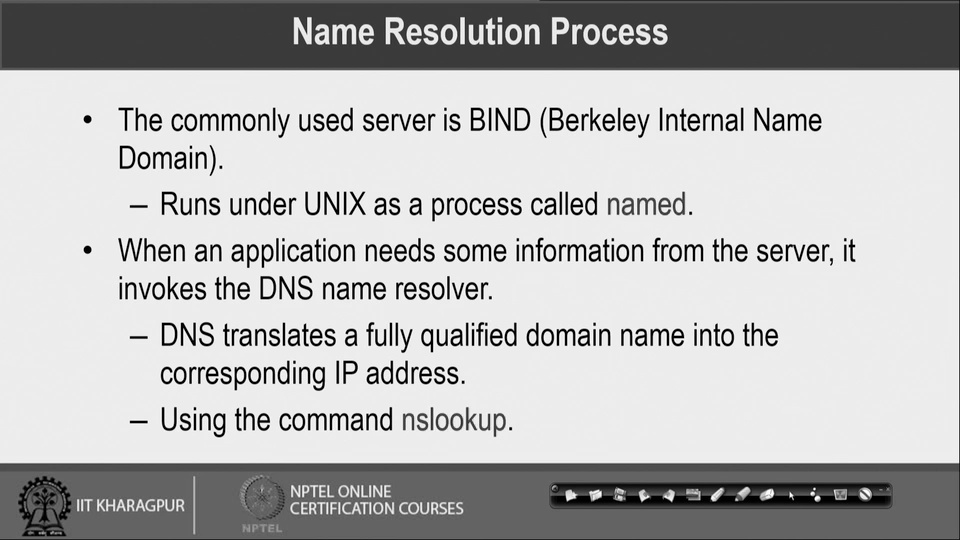
\includegraphics[width=\linewidth]{Presentation_Image/subtopic.jpg}
	\end{subfigure}
	\caption{Subtopic}
\end{figure}
\end{frame}
%%%%%%%%%%%%%%%%%%%%%%%%%%%%%%%%%%%%%%%%%%%%%%%%%%%%%%%%%%%%%%%%%%%%%%%%%%%%%%%%%%%%%%%%%

\begin{frame}
\frametitle{Slide Extraction}

\begin{itemize}
	\item Convert all frame to gray to make it two dimensional.
	\item Create canny edge for each frame.
	\item Calculate MSE, Manhattan Distance and Euclidean Distance between consecutive frames.
	\item Plot graph of two consecutive frame on different measures like MSE, Manhattan Distance and Euclidean Distance.
	\item Choose threshold based on above plots.
	\item Store frame if that frame crossed chosen threshold
\end{itemize}

\end{frame}

%%%%%%%%%%%%%%%%%%%%%%%%%%%%%%%%%%%%%%%%%%%%%%%%%%%%%%%%%%%%%%%%%%%%%%%%%%%%%%%%%%%%%%%%%%%%%%%%%%
\begin{frame}
\frametitle{Slide Exraction Approach}
\begin{figure}
	\centering
	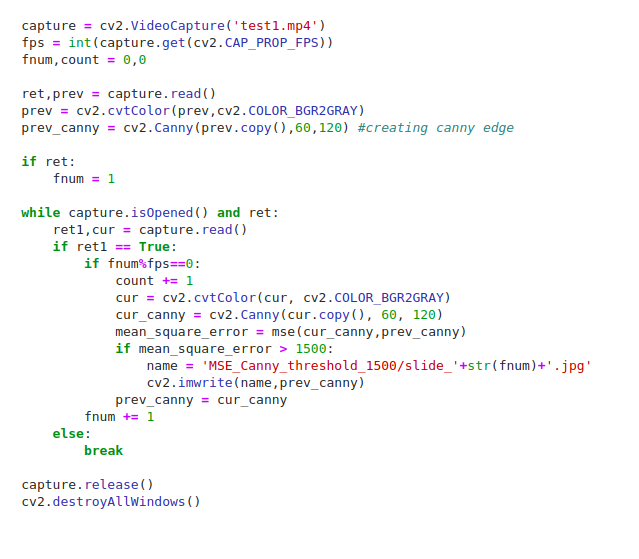
\includegraphics[width=0.8\linewidth]{Presentation_Image/slide_extraction_code}
\end{figure}	
\end{frame}
%%%%%%%%%%%%%%%%%%%%%%%%%%%%%%%%%%%%%%%%%%%%%%%%%%%%%%%%%%%%%%%%%%%%%%%%%%%%%%%%%%%%%%%%%%%%%%%%%%%%

\begin{frame}
\frametitle{Canny Edge Snapshot}
\begin{figure}[h!]
	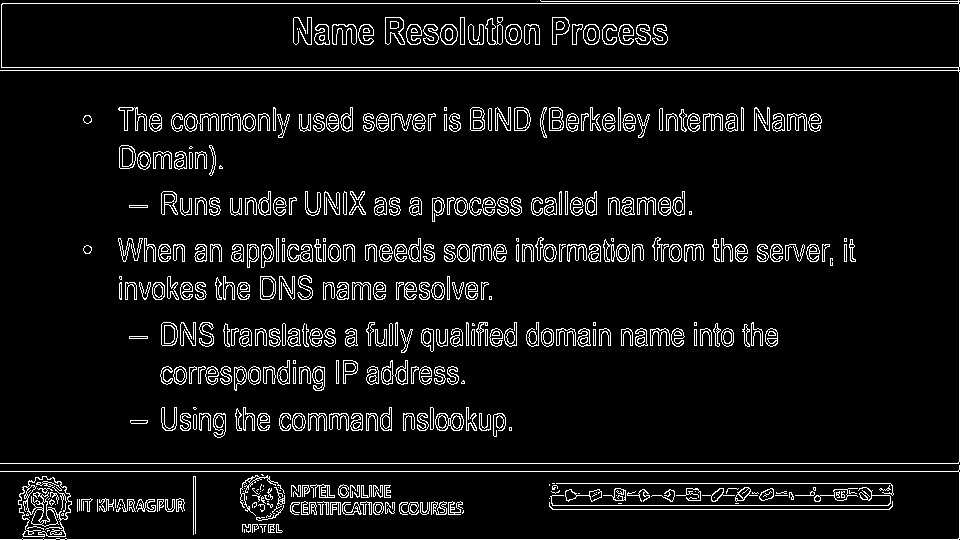
\includegraphics[width=\linewidth]{Presentation_Image/Canny.jpg}
\end{figure}
\end{frame}

%%%%%%%%%%%%%%%%%%%%%%%%%%%%%%%%%%%%%%%%%%%%%%%%%%%%%%%%%%%%%%%%%%%%%%%%%%%%%%%%%%%%%%%%%%%%%


%%%%%%%%%%%%%%%%%%%%%%%%%%%%%%%%%%%%%%%%%%%%%%%%%%%%%%%%%%%%%%%%%%%%%%%%%%%%%%%%%%%%%%%%%%
\begin{frame}
\frametitle{Mean Square Error Plot}
\begin{figure}[h!]
	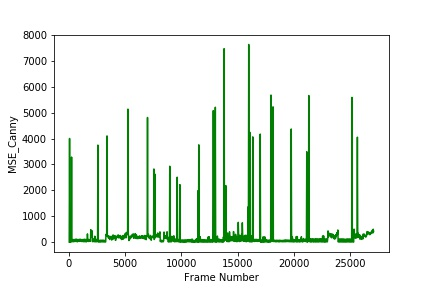
\includegraphics[width=\linewidth]{Presentation_Image/MSE_Canny.jpeg}
\end{figure}
\end{frame}

%%%%%%%%%%%%%%%%%%%%%%%%%%%%%%%%%%%%%%%%%%%%%%%%%%%%%%%%%%%%%%%%%%%%%%%%%%%%%%%%%%%%%%%%%%
\begin{frame}
\frametitle{Manhattan Distance Plot}
\begin{figure}[h!]
	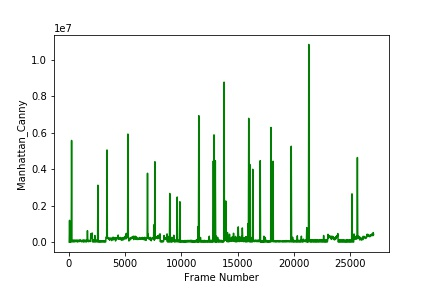
\includegraphics[width=\linewidth]{Presentation_Image/Manhattan_Canny.jpeg}
\end{figure}
\end{frame}

%%%%%%%%%%%%%%%%%%%%%%%%%%%%%%%%%%%%%%%%%%%%%%%%%%%%%%%%%%%%%%%%%%%%%%%%%%%%%%%%%%%%%%%%%%%
\begin{frame}
\frametitle{Euclidean Distance Plot}
\begin{figure}[h!]
	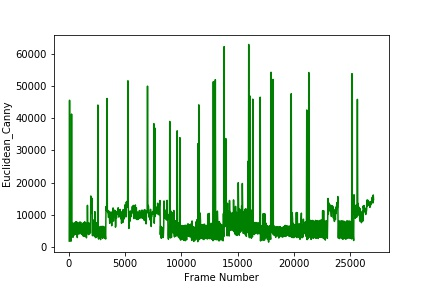
\includegraphics[width=\linewidth]{Presentation_Image/Euclidean_Canny.jpeg}
\end{figure}
\end{frame}

%%%%%%%%%%%%%%%%%%%%%%%%%%%%%%%%%%%%%%%%%%%%%%%%%%%%%%%%%%%%%%%%%%%%%%%%%%%%%%%%%%%%%%%%%%
\section{Result}
\begin{frame}
\frametitle{Result}
	\begin{itemize}
		\item Result is for same video with different threshold for diffrent measure.
	\end{itemize}
% Please add the following required packages to your document preamble:
% \usepackage{multirow}
\begin{table}[]
	\begin{tabular}{|c|c|c|c|c|}
		\hline
		\textbf{Measure} & \textbf{Threshold} & \textbf{\begin{tabular}[c]{@{}c@{}}No\\ of \\ Slides\end{tabular}} & \textbf{\begin{tabular}[c]{@{}c@{}}No of Slides \\ Detected\end{tabular}} & \textbf{\begin{tabular}[c]{@{}c@{}}No of Slides \\ Correctly \\ detected\end{tabular}} \\ \hline
		\multirow{3}{*}{\textbf{\begin{tabular}[c]{@{}c@{}}Mean \\ Square Error\end{tabular}}} & 1100 & 29 & 31 & 29 \\ \cline{2-5} 
		& 1500 & 29 & 29 & 29 \\ \cline{2-5} 
		& 2000 & 29 & 28 & 28 \\ \hline
		\multirow{3}{*}{\textbf{\begin{tabular}[c]{@{}c@{}}Manhattan \\ Distance\end{tabular}}} & 800000 & 29 & 29 & 28 \\ \cline{2-5} 
		& 1000000 & 29 & 27 & 26 \\ \cline{2-5} 
		& 2000000 & 29 & 25 & 25 \\ \hline
		\multirow{3}{*}{\textbf{\begin{tabular}[c]{@{}c@{}}Euclidean \\ Distance\end{tabular}}} & 20000 & 29 & 31 & 29 \\ \cline{2-5} 
		& 30000 & 29 & 28 & 28 \\ \cline{2-5} 
		& 35000 & 29 & 26 & 26 \\ \hline
	\end{tabular}
\end{table}

\end{frame}
%%%%%%%%%%%%%%%%%%%%%%%%%%%%%%%%%%%%%%%%%%%%%%%%%%%%%%%%%%%%%%%%%%%%%%%%%%%%%%%%%%%%%%%%%%%
\section{Topic/Subtopic}
\begin{frame}
\frametitle{Topic vs Subtopic}
	\begin{itemize}
		\item Blue region is for Topic and Green region is for subtopic.
		\item OCR will be performed on respective region.
	\end{itemize}
	\begin{figure}[h!]
		\begin{subfigure}[b]{0.5\textwidth}
			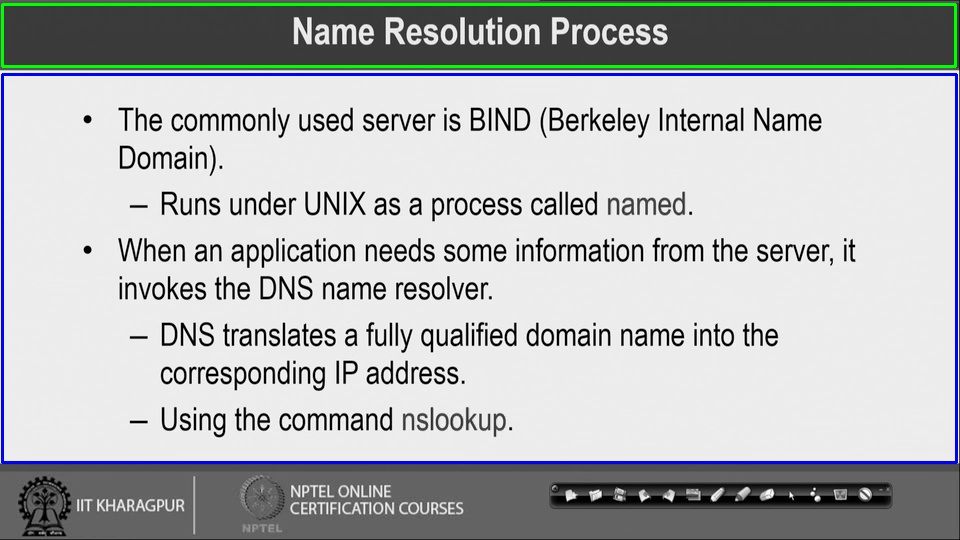
\includegraphics[width=0.95\linewidth]{Presentation_Image/Topic1.jpg}
			\caption{Subtopic}
			\label{fig:subtopic}
		\end{subfigure}%
		\begin{subfigure}[b]{0.5\textwidth}
			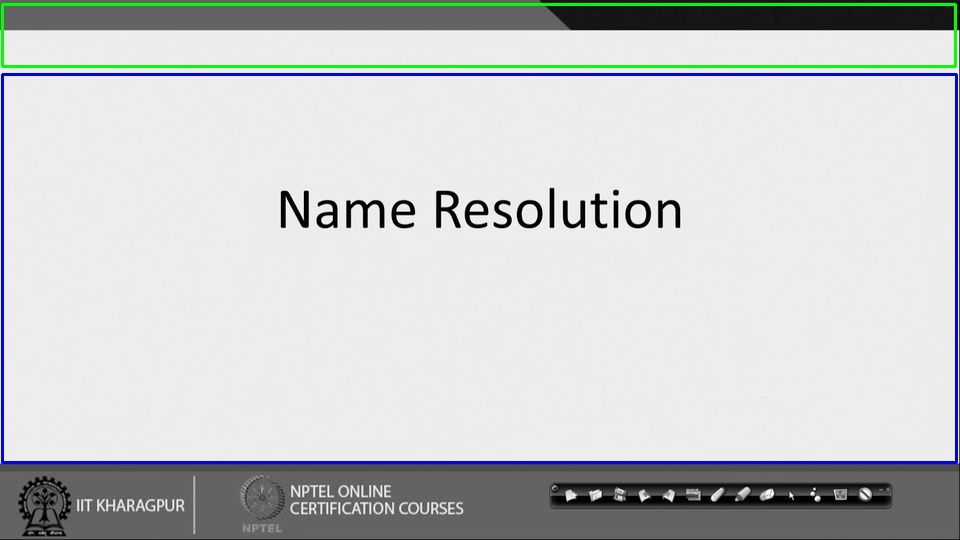
\includegraphics[width=0.95\linewidth]{Presentation_Image/Topic2.jpg}
			\caption{Topic}
			\label{fig:topic}
		\end{subfigure}%
	\end{figure}
\end{frame}
%%%%%%%%%%%%%%%%%%%%%%%%%%%%%%%%%%%%%%%%%%%%%%%%%%%%%%%%%%%%%%%%%%%%%%%%%%%%%%%%%%%%%%%%%
\section{Conclusion}
\begin{frame}
\frametitle{Conclusion }

	\begin{itemize}
		\item Course presentation should be consistent. Latex based would be preferrable.
		\item Manual fine tuning of threshold is required.
		\item Region for Topic/Subtopic is dependent on slide format.
		\item Need to run on different lecture to see the effectiveness of the method.
	\end{itemize}

\end{frame}
%%%%%%%%%%%%%%%%%%%%%%%%%%%%%%%%%%%%%%%%%%%%%%%%%%%%%%%%%%%%%%%%%%%%%%%%%%%%%%%%%%%%%%%%%


\section{Future Work}
\begin{frame}
\frametitle{Future Work }
\begin{itemize}
	\item We will analyse on different course where presentation is consistent.
	\item Topic/Subtopic selection based on text extraction(OCR) of Topic/Subtopic area. 
	\item Exploration of DNN based approach.
	
\end{itemize}
\end{frame}
%%%%%%%%%%%%%%%%%%%%%%%%%%%%%%%%%%%%%%%%%%%%%%%%%%%%%%%%%%%%%%%%%%%%%%%%%%%%%%%%%%%%%%%%%

\begin{frame}[allowframebreaks]{References}    
\bibliographystyle{IEEEtran}    %apalike, plainnat, amsalpha, IEEEtran, ieeetr
\bibliography{Ref}
\end{frame}


\begin{frame}
\Huge{\centerline{Thank You}}
\end{frame}








%----------------------------------------------------------------------------------------

\end{document} 
